\documentclass[10pt,a4paper]{book}
\usepackage[utf8]{inputenc}
\usepackage{amsmath}
\usepackage{amsfonts}
\usepackage{amssymb}
\usepackage{minted}
\definecolor{mygray}{gray}{0.9}
\usepackage{graphicx}
\usepackage{hyperref}
\usepackage{enumitem}
\author{Nicolò Fornari}
\title{Security testing}
\definecolor{mygray}{gray}{0.9}
\begin{document}
%\maketitle
\chapter{Assembly}
\section{Registers}
\textbf{What are registers for?}
\begin{itemize}[noitemsep,nolistsep]
\item Store instructions
\item Store result of operations
\item Manipulate data in them (shift registers)
\end{itemize}

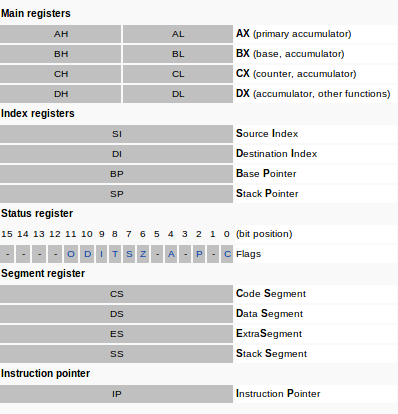
\includegraphics[scale=0.6]{registers.png}

\textbf{Why EAX,EBX,ECX?}
Registers AL,AH,BL,BH,CL,CH,DL,DH are of 16 bits each and can be used in pairs: AX, BX, CX, DX
\newpage
\section{Hello world}
\begin{minted}[
bgcolor=mygray,
]{as}
section .data
	hello:     db 'Hello world!',10    ; 
	helloLen:  equ \$-hello             ; length 
	                                   ; to be explained

section .text
	global _start

_start:
	mov eax,4            ; (sys_write)
	mov ebx,1            ; standard output
	mov ecx,hello        ; offset into in ecx
	mov edx,helloLen     ; helloLen is a constant
	                     ;  
	int 80h              ; Call the kernel

	mov eax,1            ; (sys_exit)
	mov ebx,0            ; return code of 0 (no error)
	int 80h
\end{minted}
\\\\
Then in the terminal:\\\\
\begin{minted}[
bgcolor=mygray,
]{as}
nasm -f elf hello.asm
ld -m elf_i386 -s -o hello hello.o
\end{minted}
\\\\
Note that the elf\_i386 is necessary as we are writing 32 bit assembly code in a 64 bit architecture.
\newpage
\section{Introducing concepts with an example}
Let's look at some short code and describe what it does. Please note that it's pseudocode, it's not made for a specific architecture or language and various symbols can differ, the principle however, remains the same\\\\
\begin{minted}[
bgcolor=mygray,
]{as}
MOV A, 2000
LOOP:
ADD A, #5
JNL A, #200, LOOP
MOV 2001, A
\end{minted}
\\\\
The first instruction will move the number from the memory cell with address 2000 to a register A - it's a temporary location, where the processor stores numbers. It can have many registers like this. The second line contains something called a \textbf{label}: it's not an instruction, it's simply a mark in the source code that we may use later.\\\\
On the third line, there's an ADD instruction, which adds two numbers together. The operands are register A and number 5 (the \# mark before tells the assembler that it's number five, not a number in the memory cell with address 5). And remember? We stored the value from memory location 2000 in the A register, so whatever the value is, this instruction will add the number 5 to it.\\\\
The following instruction is called a \textbf{conditional jump}: the processor will test some condition and based on the result, it will jump or not. In this case, the condition is whether a given number is not larger than another one (JNL = Jump (if) Not Larger). The number being compared is the number in register A, with the number 200 (again, mark \# means that it's a direct number, not a number from the memory location with address 200). In this case, the number in A is smaller than 200 (thus not larger than 200 - condition is true), the processor will make a jump at the instruction specified by the third operand, and this is where our label comes in: the assembler tool (the translator) will replace "LOOP" with the memory address of the instruction right after this mark.\\\\
So if the number is smaller, the processor will jump back to the instruction ADD and again add value 5 to the number A (which is already larger from the previous calculation) and then get back to the JNL instruction. If the number is still smaller than 200, it will jump back again; however, if it is larger, then the condition won't be true anymore, so no jump occurs and the following instruction gets executed. This one moves value from register A to the memory cell with address 2001, basically storing the resulting number there. It's important to add, that the memory cell with address 2000 still contains the original value, because we created a copy of it in register A, we didn't modify the original.
\newpage
\section{x86 instructions}
Here we list very few  x86 instructions
\begin{itemize}
\item Boolean: AND, OR XOR,NOT
\item Stack Related: PUSH,POP
\item Shift operations: a lot of them
\item MOV (copies data from one location to another)
\item JMP (transfers the flow of execution by changing the instruction pointer register)
\item NOP (no operation)
\item INT (call to interrupt)
\item Jcc (jump if condition)
\end{itemize}
\section{Linux system calls}
Linux system calls can be used in an assembly program with the following steps:
\begin{itemize}
\item Put the system call number in the EAX register
\item Store the arguments to the system calls in the registers EBX,ECX,etc.
\item Call the relevant interrupt (80h)
\item The result is usually returned in the EAX register 
\end{itemize}
\begin{tabular}{|c|c|c|}
\hline 
\%eax & Name & \%ebx \\ 
\hline 
1 & sys\_exit & int \\ 
\hline 
2 & sys\_fork & struct pt\_regs \\ 
\hline 
3 & sys\_read & unsigned int \\ 
\hline 
4 & sys\_write & unsigned int \\ 
\hline 
5 & sys\_open & const char * \\ 
\hline 
6 & sys\_close & unsigned int \\ 
\hline 
\end{tabular} 
\newpage
\section{References}
\begin{enumerate}
\item \url{https://www.quora.com/What-is-an-intuitive-explanation-of-how-CPU-registers-work}
\item \url{http://stackoverflow.com/questions/2545192/what-does-x-mean-in-eax-ebx-ecx-in-assembly}
\item \url{http://docs.cs.up.ac.za/programming/asm/derick_tut/}
\item \url{http://www.codeproject.com/Articles/315505/How-processor-assembler-and-programming-languages}
\item \url{https://en.wikipedia.org/wiki/X86_instruction_listings}
\item \url{http://www.tutorialspoint.com/assembly_programming/assembly_system_calls.htm}
\end{enumerate}

\end{document}
